\chapter{Parameter Sensitivity}\label{chp:chp4}

%\begin{flushright}
%  {\em QUOTE GOES HERE }\\
%
%\ \
%
%\normalsize
%{AUTHOR}  
%\end{flushright}


\label{ps}

\begin{figure}
\includegraphics[trim =87 30 6 15,clip=true,scale=0.45]{chapters/chapter4/images/params/D/newDall}
\caption{Set of models with $i(r) \propto r^{-2\beta}$ for $\beta=1.0$ (left), $\beta=1.5$ (middle) or $\beta=2.0$ (right), $\omega=0$, 
$R_{in}/R_{out}=0.2$, $v(r) \propto r$ and $v_{max}=1$ illustrating the effects of varying 
$\tau$.  Peak fluxes are scaled to unity.}
\label{bt}
\end{figure}

\begin{figure}
\includegraphics[trim =80 60 40 15,clip=true,scale=0.45]{chapters/chapter4/images/params/C/C_all}
\caption{Set of models with $i(r) \propto r^{-4}$ (i.e. $\beta=2.0$), $R_{in}/R_{out}=0.2$, $v(r) \propto r$  
and $v_{max}=1$ illustrating the effects of varying $\tau$ and $\omega$. 
Peak fluxes are scaled to unity.}
\label{wt}
\end{figure}


It is of general interest to establish potential diagnostic signatures in 
the line profiles of supernovae and their remnants in order to trace dust 
formation more effectively.  We here discuss the effects of the main 
parameters of interest, namely:

\begin{itemize}
\item $V_{max}$
\item $R_{in}/R_{out}$
\item $\beta$, where $\rho \propto r^{-\beta}$
\item albedo $\omega$ 
\item optical depth  $\tau$
\end{itemize}


\section{The maximum line velocity $V_{max}$}

The maximum velocity is defined as the velocity at the outer edges of 
the line emitting region for a given line.  The 
maximum velocity may vary between different spectral lines or doublets due 
to different locations of  species having differing ionization 
thresholds.  Clearly, the larger the maximum velocity used the wider the 
profile becomes.  To some extent therefore the steepness of the density 
profile and the maximum velocity can act to counter each other since a steeper 
density profile narrows the profile (see Section \ref{beta}).  The shape 
of the wings of the profiles, however, generally preclude much degeneracy 
in this aspect - the overall shape of the line profile can be used to determine the 
exponent of the density profile to within a relatively small range.

More important is the effect that the maximum velocity has on the overall 
optical depth.  Since the overall volume of the ejecta is determined 
solely by the maximum velocity and the ratio of the inner and outer radii, 
the total optical depth to which the radiation is exposed can be greatly 
affected by even a relatively small change in the maximum velocity.  
Practically speaking, the maximum velocity can usually be fairly well determined 
from the observations (identified as the point where the flux vanishes 
on the blue side) and may be further constrained through modelling.

\section{The ejecta radius ratio $R_{in}/R_{out}$}

As already discussed in Section \ref{analytics}, the width of the flat top 
is determined solely by the ratio of the inner and outer radii, the 
exponent of the velocity profile and the maximum velocity.  We to 
assume that the velocity profile takes the form $v \propto r$ from 
just a few months after the explosion as the supernova is in free 
expansion.  For this case, $R_{in}/R_{out}$ is given by

\begin{equation}
\frac{R_{in}}{R_{out}}=\frac{V_{min}}{V_{max}}
\end{equation}

\noindent where it is often possible to constrain $V_{min}$ and $V_{max}$ 
to a relatively narrow range simply from the observed line profile.

The majority of spectral lines emitted from supernovae and supernova 
remnants are expected to have a flat top before dust attenuation effects since it is rare for these 
objects to form a completely filled nebula.  However, even a very small amount of 
dust attenuation may result in the line profile appearing to be smoothed at its 
peak.

\begin{figure}

\begin{subfigure}{1\textwidth}
\centering
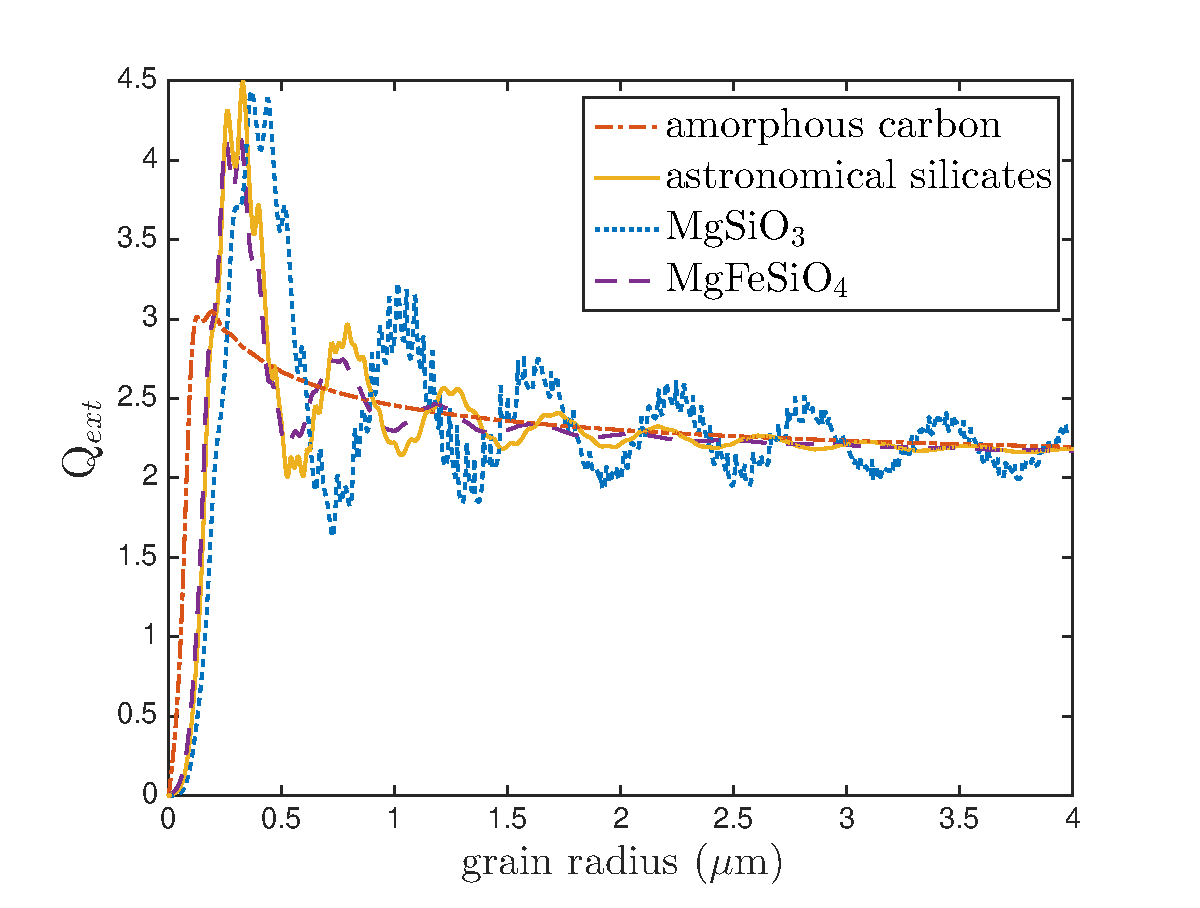
\includegraphics[trim =37 10 45 15,clip=true,scale=0.75]{chapters/chapter4/images/Qext_grainsize_upto4}
\end{subfigure}\\[1ex]
\begin{subfigure}{\textwidth}
\centering
\includegraphics[trim =35 10 45 15,clip=true,scale=0.75]{chapters/chapter4/images/Qext_grainsize_upto4_log}
\end{subfigure}
\caption{Variation of extinction efficiency ($Q_{ext}$) with grain size for amorphous carbon and silicates using Mie theory at $\lambda = 658 \mu $m. Optical constants are from \citet{Zubko1996} and \citet{Draine1984}. A linear scale is presented on the top and a log scale on the bottom.}
\label{Qext_grain}
\end{figure}

\begin{figure}
\begin{subfigure}{1\textwidth}
\centering
\includegraphics[trim =37 10 45 15,clip=true,scale=0.75]{chapters/chapter4/images/albedo_grainsize_upto4}
\end{subfigure}\\[1ex]
\begin{subfigure}{1\textwidth}
\centering
\includegraphics[trim =35 10 45 15,clip=true,scale=0.75]{chapters/chapter4/images/albedo_grainsize_upto4_log}
\end{subfigure}
\caption{Variation of albedo with grain size for amorphous carbon and silicates using Mie theory at $\lambda = 658 \mu $m. Optical constants are from \citet{Zubko1996} and \citet{Draine1984}. A linear scale is presented on the top and a log scale on the bottom.}
\label{albedo_grain}
\end{figure}

The effects of dust on a line profile for $R_{in}/R_{out}=0$ as opposed 
to a detached shell, is shown in Figure \ref{fig:analytics}.  
The effects of line scatting from moving dust grains are evidenced 
by the presence of an extended red scattering wing beyond $V_{max}$ as shown in Figure \ref{wt}. 
All profiles have been scaled to unity flux at their peaks.



\section{The dust optical depth $\tau$ (detached shell case)}
\label{tau}

As expected, Figures \ref{bt} and \ref{wt} show greater attenuation of the original line profile on 
the red side.  The profiles are most revealing at lower 
dust optical depths.  The effects of the asymmetric absorption can be seen in 
different sections of the profiles.  The region of the profile that is 
most clearly affected by dust absorption is the flat-topped region.  A 
small amount of absorption in this region results in a skewed profile, 
with a fraction of the flat-topped section removed.  The peak becomes 
blue-shifted as a result, but only to the original value of $-V_{min}$, the minimum 
velocity corresponding to $R_{in}$. In addition to the attenuation in this region, 
the red wing of the profile is also somewhat reduced, and the blue wing 
somewhat increased relative to their original symmetric positions.  The 
result is a relatively ``jagged'' looking profile, often with sharp changes 
at $\pm V_{min}$.  The profile is generally asymmetric, although the 
degree of absorption in the flat-topped region may sometimes make it seem 
as though the profile is in fact symmetric and uniformly blue-shifted (see 
Section \ref{asym} for further discussion).

At high dust optical depths the entire profile is shifted to the blue and the 
peak moves beyond $-V_{min}$ further into the blue.  The 
profiles also become more smooth.  A set of models showing 
the effects of varying optical depths for different density profiles and 
dust albedos are presented in Figures \ref{bt} and \ref{wt}.


\section{The dust albedo $\omega$}
\label{omega}

In the past, there has largely been a focus on the effects of absorption by dust 
on the shapes of line profiles and less attention has been paid to the 
potential effects of scattering by dust.  In fact, line profiles 
can be significantly affected by scattering of radiation.  Not only does 
repeated scattering of photons increase the number of potential 
opportunities for a given photon to be absorbed but it also results in 
continuous shifting of the frequency of the photon to the red.  The photon 
must do work on the expanding shell of dust in order to escape and thus 
many of the photons are reprocessed beyond the theoretical maximum 
velocity on the red side of the profile.  The result can be a substantial, 
extended wing on the red side of the line.  In the case of strong 
dust scattering, this can result in an asymmetric profile that is the opposite 
of that normally expected with the majority of the emission on the 
\textit{red} side.  The peak however, remains blue-shifted (see the bottom right panel on Figure \ref{wt} for an example).  
For the line profile to exhibit this feature requires the dust to be a 
nearly perfect scatterer and it is therefore unlikely that profiles of this sort will be
frequently observed.  See Figure \ref{wt} for a fuller illustration of the variation
with $\omega$ and $\tau$.

The implications of this result in relation to the use of line profiles as 
a diagnostic for tracing dust formation in supernova ejecta 
are discussed further in Section \ref{asym}.


\section{Density profile $\rho \propto r^{-2\beta}$}
\label{beta}

Whilst the density profile of the dust may have some effect on the 
resulting profiles, it is the initial emissivity profile (dependent on the 
dust density profile) that has greatest effect on the resulting shape of 
the line profile.

In general, the steeper the emissivity distribution, the narrower the line 
profile becomes.  The sides of the line profile may become almost straight 
for a very steep distribution since the majority of the emission then 
comes from a very narrow velocity range.  For a flat-topped profile of 
fixed width this approximates the square profile produced in the case of 
an emitting shell with constant velocity.

The dependence of the shape of the line profile in the optically thin dust case 
is described in Section \ref{analytics}.  However, the density profile 
also plays a significant role where there is even a small amount of 
absorption.  As previously discussed, at relatively small optical depths, 
a section of the flat-topped region is removed resulting in a peak at 
$-V_{min}$.  The shape of the profile in this region is significantly 
affected by the density profile.  Shallow density profiles (low $\beta$) produce a virtually 
linear variation in flux between $-V_{min}$ and $+V_{min}$.  For a fixed dust
optical depth, the steeper the distribution becomes, the more concave the 
profile becomes between $-V_{min}$ and $+V_{min}$, ultimately resulting in 
a clear shoulder to the profile at $+V_{min}$.  For extremely steep density
distributions this can result in a double peaked profile with 
trough to the red of $V=0$.  A illustration of the effects of variation of 
$\beta$ with $\tau$ on the profiles is shown in Figure \ref{bt}.

\section{Inferring properties of the dust from the models}

The presence of an extended red wing at large positive velocities in 
combination with increased extinction on the red side at smaller positive 
velocities can allow the values of $\tau$ and $\omega$ to be well 
constrained.  In this case it is possible to translate these values into a 
dust mass and average grain size for a given species or combination of 
species using optical properties Mie theory (see Figures 
\ref{albedo_grain} and \ref{Qext_grain}).  In fact, it is the dust mass and average grain size 
that is varied within the code for a specified species or combination of 
species.  It is therefore important to note that the use of different 
optical properties may substantially alter the inferred optical depths and 
albedos for a given species of specific grain size as has been noted 
previously (e.g. \citet{Owen2015}).



For amorphous carbon, the larger the grain size used the larger the albedo 
and the smaller the cross-section of absorption.  Larger masses of dust 
are therefore required to fit the same degree of absorption if a larger 
grain size is used.  This is in contrast to SED radiative transfer 
modelling where larger grain sizes generally result in less dust being 
required to fit the IR portion of the SED (W15).  These two techniques in 
tandem may therefore give excellent limits on grain sizes for different 
species or combinations thereof.

\begin{figure}
\begin{subfigure}{0.5\textwidth}
\includegraphics[trim =30 31 45 0,clip=true,scale=0.45]{chapters/chapter4/images/dustdep/a0_001_opt_thin_HaHbPad}
\end{subfigure}
\hspace{4mm}
\begin{subfigure}{0.5\textwidth}
\includegraphics[trim =59 31 45 0,clip=true,scale=0.45]{chapters/chapter4/images/dustdep/a0_001_opt_thick_HaHbPad}
\end{subfigure} \\[1ex]

\begin{subfigure}{0.5\textwidth}

\includegraphics[trim =30 31 45 0,clip=true,scale=0.45]{chapters/chapter4/images/dustdep/a0_1_opt_thin_HaHbPad}
\end{subfigure}
\hspace{4mm}
\begin{subfigure}{0.5\textwidth}
\includegraphics[trim =59 31 45 0,clip=true,scale=0.45]{chapters/chapter4/images/dustdep/a0_1_opt_thick_HaHbPad}
\end{subfigure} \\[1ex]

\begin{subfigure}{0.5\textwidth}
\includegraphics[trim =30 0 45 15,clip=true,scale=0.45]{chapters/chapter4/images/dustdep/a1_opt_thin_HaHbPad}
\end{subfigure}
\hspace{3mm}
\begin{subfigure}{0.5\textwidth}
\includegraphics[trim =51 0 45 15,clip=true,scale=0.45]{chapters/chapter4/images/dustdep/a1_opt_thick_HaHbPad}
\end{subfigure}
\caption{Model line profiles for H$\alpha$ (6563\AA\ in red), H$\beta$ (4861\AA\ in yellow) and Pa$\delta$ (10049\AA\ in blue) for optically thin and  optically thick cases on the left-hand side and right-hand side respectively.  All models adopted density profile $\rho(r) \propto r^{-4}$ (i.e. $\beta = 2$), velocity profiles $v(r) \propto r$ and radii ratio $R_{in}/R_{out}=0.2$.  The grain radii used were $a=0.001~\mu$m (top), $a=0.1~\mu$m (middle) and $a=1.0~\mu$m (bottom). All the above models used amorphous carbon.}
\label{wav_dep}
\end{figure}

\begin{figure}
\begin{subfigure}{\textwidth}
\centering
\includegraphics[trim =30 30 45 25,clip=true,scale=0.55]{chapters/chapter4/images/Qabs_a0_001}
\end{subfigure} \\[0.5ex]

\begin{subfigure}{\textwidth}
\centering

\includegraphics[trim =30 30 45 25,clip=true,scale=0.55]{chapters/chapter4/images/Qabs_a0_1} 
\end{subfigure} \\[0.5ex]

\begin{subfigure}{\textwidth}
\centering
\includegraphics[trim =30 10 45 25,clip=true,scale=0.55]{chapters/chapter4/images/Qabs_a1_0}
\end{subfigure}
\caption{The variation of amorphous carbon dust absorption efficiency with grain size. The grain radii plotted are $a=0.001~\mu$m (top), $a=0.1~\mu$m (middle) and $a=1.0~\mu$m (bottom).  The vertical lines mark the wavelengths of H$\alpha$ (6563\AA\ in red), H$\beta$ (4861\AA\ in yellow) and Pa$\delta$ (10049\AA\ in blue).}
\label{wav_dep2}
\end{figure}






\section{Observable signatures of dust in line profiles}
\label{asym}

The greater the dust optical depth, the more attenuation of the line 
is observed.  As expected, the red side of the profile suffers a greater 
degree of absorption than the blue side.  The resulting asymmetry is 
somewhat more complex than perhaps previously thought however.  Dust has 
repeatedly been cited as the agent responsible for the apparent 
blue-shifting of line profiles in supernovae in the manner of the profiles 
presented in Figure \ref{fig:Lucy}.  That is, relatively high optical 
depths result in an overall shift of the entire profile towards the blue.

In practice a relatively large optical depth ($\tau \approx 2$) is 
required to actively shift the peak of the profile bluewards of its natural 
$V_{min}$ value corresponding to the velocity at the inner radius of the shell.  In most cases it seems more likely that the dust
may not be optically thick and the blue-shifting of the peak of the profile is 
likely a result of attenuation in the flat-topped section (close to 
$R_{in}$).  The peak would therefore tend to be located at $-V_{min}$.

Since dust absorption is wavelength dependent for $2\pi a < \lambda$, one might expect the 
position of the peak flux to be dependent on the wavelength of the line being 
considered.  The relationship between the locations of the peaks 
of profiles and their wavelength has been discussed by several authors in 
relation to dust formation \citep{Smith2012, Fransson2013, Gall2014}.  We 
note here that whilst this may occur in cases of high dust 
optical depth, this is not necessarily likely to be seen in the ejecta of 
most supernovae.  The wavelength-dependence of dust absorption instead 
can result in differing degrees of extinction in the flat-topped region of 
each profile but still leave the peak at its blue-shifted position of 
$-V_{min}$.  Of course, the value of $V_{min}$ may be different for 
different species.  However, if this is the case then there would be no 
reason to expect a variation in the position of the peak of profiles to be 
correlated with the wavelength dependence of dust.  Rather one would 
expect it potentially to trace the location of different ions within the ejecta. 
However, for lines from the same ion, for example the Balmer and Paschen lines of HI,
we might expect to see peaks at the same position but differing degrees of absorption.
At high resolutions, it might be possible to detect differences in the shape of the line 
profiles, particularly between $-V_{min}$ and $+V_{min}$ where the steepness of the 
incline traces the degree of dust absorption.  This can be seen in Figure \ref{wav_dep} 
where we illustrate the effects of the wavelength dependence of dust absorption for 
three lines, H$\alpha$ (6563\AA), H$\beta$ (4861\AA) and Pa$\delta$ (10049\AA).  
All lines were modelled using three different grain sizes and in both optically thin and 
thick cases.  We also show the variation of the absorption cross-section with 
wavelength at three different grain sizes in Figure \ref{wav_dep2}.

The attenuation of the flat-topped region is also often such that it can 
be hard to discern a difference in slope between the attenuated 
section between $-V_{min}$ and $+V_{min}$ and the slope of the wing for 
$V>+V_{min}$, particularly in circumstances where data is of poor 
resolution or has a poor signal-to-noise ratio.  Even in the case of 
excellent data, it may be easy to overlook these particular features or to 
dismiss them as natural fluctuations in the geometry of the ejecta rather than 
that they may be a product of dust absorption effects.

The greater attenuation of radiation received from the receding portion of 
the ejecta results in an asymmetry of the line profile whereby the 
majority of the observed emission is located bluewards of the peak.  
However, the effects of repeated dust scattering events within the 
ejecta can serve to counter this asymmetry.  Even in the case of dust grains 
with a relatively low albedo, a surprisingly persistent wing on the red 
side of the profile is seen, often beyond the maximum theoretical velocity 
of the emitting region.  For higher albedos this can actively result in a 
shift in the overall asymmetry of the profile, with the majority of the 
emission being emitted redwards of the peak, though the peak itself 
remains blue-shifted.

This effect is obviously analogous to that of electron scattering which 
also produces a significant red wing in line profiles \citep{Hillier1991, 
Auer1972b}. This is an important consideration in both modelling and 
analysis of spectral line profiles.  DAMOCLES has the capacity to include 
a basic electron scattering mechanism in order to assess the possibility 
that any observed red wing might be produced by electron scattering rather 
than dust scattering.  The red wing observed in line profiles is an 
excellent diagnostic for determining the overall dust albedo and it is 
therefore important to establish whether this feature is due to 
electron or dust scattering or a combination of the two.

The combination of relatively low optical depths, initially flat-topped 
profiles, greater attenuation on the blue side with increased flux on the 
red side due to scattering can result in a profile that ends up appearing 
almost symmetrical, particularly if 
contaminants, such as narrow lines or blending with other broad lines, are 
present or if the resolution of the data is low.  The potential for apparently 
symmetrical profiles that appear to have been uniformly blue-shifted 
should be noted (see Figures \ref{bt} and \ref{wt} for examples of this).



\section{The effect of a grain size distribution}
\label{gs_distn}
It is important to consider the potential effect on the dust mass of modelling a grain size distribution instead of a single grain size.  For a grain size distribution the overall extinction cross section, $C_{ext}$, at a given wavelength is calculated as

\[ C_{ext}=\int^{a_{max}}_{a_{min}} Q_{ext}(a) n(a) \pi a^2 da \]

where $Q_{ext}(a)$ is the extinction efficiency for a grain size $a$ and $n(a)$ is the number of grains with size $a$. The overall extinction efficiency is then

\[ Q_{ext} = \frac{C_{ext}}{ \int^{a_{max}}_{a_{min}} n(a) \pi a^2 da} \]
 
The scattering cross-section $Q_{sca}$ is similarly calculated.  As a result of these calculations, there is rarely a single grain size that has the same albedo and extinction efficiency as a size distribution.  Modelling a size distribution may therefore alter the deduced dust mass.  Since the models are only sensitive to the optical depth and the albedo, however, it is not possible to deduce the grain size range or distribution and only single grain sizes are investigated (as presented above).

Whilst this apparently limits the scope of the results, it is important to consider the extent to which considering grain size distributions would alter the derived dust masses.  By considering a number of grain size ranges and adopting a power law distribution with a variable exponent, we may gain some insight into the effects of adopting a distribution rather than a single size.  For the classical MRN power law ($n(a) \propto a^{-3.5}$) with a wide grain size range ($a_{min} = 0.001 \mu$m to $a_{max} = 4.0 \mu$m) the derived albedo is much too small to reproduce the required wing seen at early epochs.  We therefore adopt an approach whereby, for a number of grain size ranges, we adjust the exponent of the distribution until the overall albedo is the same as that seen for the best fitting single grain size for the clumped distributions.  We may then approximately calculate the required dust mass as

\begin{equation}
\label{distn_conv}
M_{d}= \frac{M_s Q_{ext,s}(a_s)}{a_s} \times \frac{\int^{a_{max}}_{a_{min}} n(a) a^3 da}{\int^{a_{max}}_{a_{min}} Q_{ext}(a) n(a) a^2 da}
\end{equation}

where the subscript $s$ represents the single grain size quantities and the $d$ subscript represents quantities for the grain size distribution.  

We calculate the required dust masses for the clumped model on day 714 for a selection of distributions with varied $a_{min}$.  These are presented in Table \ref{tb_distn}.  It can be seen that in all cases, a larger dust mass is required in order to reproduce the same conditions as a single grain size.  The conversion factors presented in the table are valid for any model with grain size $a=0.6\mu$m and may therefore also be applied to the models for day 806.  We repeated the process for $a=3.5 \mu$m but found that, in order to reproduce the required albedo, the distribution had to be heavily weighted towards the larger grains and that the value of $a_{min}$ had no effect of the required dust mass.  Increasing the value of $a_{min}$ to larger values (>2$\mu$m) does not have a significant effect either.  This is because both extinction efficiency and albedo tend to a constant value with increasing grain radius and the adoption of different grain size ranges and distributions above a certain threshold therefore results in only insignificant variation in these quantities. 

\begin{table}
	%\begin{minipage}{180mm}
	\caption{Equivalent dust masses for the day 714 clumped models using grain size distributions and 100\% amorphous carbon. $f$ is factor of increase from the dust mass for the single size model ($M=7 \times 10^{-5} M_{\odot}$ with $a=0.6 \mu$m) and $p$ is the exponent of the grain size distribution $n(a) \propto a^{-p}$.}
	\label{tb_distn}
	\begin{center}
  	\begin{tabular}{@{} ccccc @{}}
    	\hline
$a_{min}$ & $a_{max}$ & $p$ & $M$ & $f$  \\%& $Q_{ext}$ \\
($\mu$m) & ($\mu$m) & & ($M_{\odot}$) & \\
\hline
0.001 & 4 & 2.45 & 1.93E-04 & 2.76 \\%& 2.13 \\
0.01 & 4 & 2.45 & 1.93E-04 & 2.76 \\%& 2.32 \\
0.05 & 4 & 2.52 & 1.84E-04 & 2.62 \\%& 2.44 \\
0.1 & 4 & 2.72 & 1.61E-04 & 2.3\\ %& 2.53 \\
0.5 & 4 & 8.2 & 7.23E-04 & 1.03 \\%& 2.61 \\

    \hline
  \end{tabular}
  \end{center}
%\end{minipage}
\end{table}

This calculation in equation \ref{distn_conv} holds only for a single wavelength and therefore is not exact for our models which obviously transport radiation over a range of wavelengths.  However, the dust masses derived using the above formula produce almost identical fits to the data as for the single grain size and therefore give an excellent suggestion of the approximate dust mass required when using a distribution.

We therefore conclude that, if a distribution of grain sizes is indeed present, the deduced dust masses are likely to be under-estimating the true mass of newly formed dust rather than overestimating it.

\section{The effect of different species}

In all of our analyses heretofore, we have considered only amorphous carbon as the species of interest.  This is in part motivated by previously published literature that suggests that, if silicates do form a fraction of the total dust mass, it is likely that that fraction is limited to approximately 15\% (W15, \citet{Ercolano2007}).  It is also partly motivated by the nature of the model; the parameters that affect the quantity of dust required in the model are the albedo and the optical depth.  There are likely many possible combinations of species and grain sizes that result in a good fit to the data.  

We consider the change in dust mass when a medium of 100\% silicates is used instead of amorphous carbon.  We use optical constants presented in \cite{Draine1984}.  In a similar manner to the approach detailed in Section \ref{gs_distn}, we may calculate the mass of silicates that is equivalent to a carbon mass for a single grain size.  We consider the albedo at the original grain size, calculate the equivalent grain size for silicates that results in the same albedo and then calculate the new dust mass by considering the change in the extinction efficiency as

\begin{equation}
M_{sil} = M_{amc} \Big( \frac{Q_{amc}}{Q_{sil}} \Big) \Big(\frac{a_{sil}}{a_{amc}}\Big) \Big(\frac{\rho_{sil}}{\rho_{amC}}\Big)
\end{equation}

Because of the nature of the variation of albedo with grain size for silicates (see Figure \ref{albedo_grain}), there is often more than one silicate grain size that will give rise to the same albedo.  We consider all the possibilities and the resulting mass conversion factors in Table \ref{tb_sil}.  In our best fitting models for days 714 and 806, using any fraction of silicates of either grain size would serve to increase the dust mass.  However, at later epochs, using some fraction of silicate dust would reduce the dust mass to potentially more than half of our estimated values. However, this is still within our predicted range and our minimum and maximum dust masses remain robust.

\begin{table}
	%\begin{minipage}{180mm}
	\caption{Equivalent dust masses for the day 714 clumped models using grain size distributions and 100\% amorphous carbon. $f$ is factor of increase from the dust mass for the single size model ($M=7 \times 10^{-5} M_{\odot}$ with $a=0.6 \mu$m) and $p$ is the exponent of the grain size distribution $n(a) \propto a^{-p}$.}
	\label{tb_sil}
	\begin{center}
  	\begin{tabular}{@{} cccccc @{}}
    	\hline
	\multicolumn{2}{c}{\textit{carbon}} && \multicolumn{2}{c}{\textit{silicates}} & \\
$a$ & $Q_{ext}$ & &$a$& $Q_{ext}$ & $f=M_{sil}/M_{amc}$ \\
\hline
0.6 & 2.60633 & &0.0583 & 0.0772 & 5.37 \\
0.6 & 2.60633 & &4 & 2.1828 & 13 \\
 \\
3.5 & 2.2129 & &0.0641 & 0.10182 & 0.65 \\
3.5 & 2.2129 & &1.02 & 2.149 & 0.49 \\
3.5 & 2.2129 & &1.376 & 2.3514 & 0.61 \\


    \hline
  \end{tabular}
  \end{center}
%\end{minipage}
\end{table}









